\documentclass[10pt]{beamer}
\usepackage{uglibeamer2}
\title{Programmation fonctionnelle}

\author{NSI2}

\begin{document}
\maketitle


\begin{frame}{}
	Tout comme la programmation récursive ou orientée objet, la \textit{programmation fonctionnelle} est un des multiples paradigmes de programmation.\\
\pause

\textsc{Python}, langage multi paradigme, autorise la programmation fonctionnelle, seule ou même combinée aux autres méthodes de programmation.\\\pause

\textit{« Une fonction est une donnée comme les autres. »}
\end{frame}



\section{Fonction comme valeur passée à une autre fonction}

\begin{frame}[fragile]{Un concept déjà rencontré}
	Nous avons déjà utilisé la fonction \mintinline{python}{sorted} de \textsc{Python} pour trier des listes suivant différents critères.\\\pause
Par exemple pour trier une liste de paires d'\mintinline{python}{int} dans l'ordre croissant suivant leur deuxième élément, on écrit ceci\pause

\inputminted{python}{scripts/sort1.py}
\end{frame}

\begin{frame}[fragile]{Analyse}
On a bel et bien passé la fonction \texttt{f} \textit{comme paramètre} à la fonction \mintinline{python}{sorted}.\\\pause
Ainsi \texttt{f} est considérée comme une variable. D'ailleurs elle a un type :\pause
\begin{minted}{python}
>>> type(f)

<class 'function'>
\end{minted}
\end{frame} 

\begin{frame}[fragile]{Un autre exemple}
La programmation fonctionnelle nous autorise à créer et utiliser des fonctions prenant d'autres fonctions comme paramètres :\pause

\inputminted{python}{scripts/func1.py}
\end{frame}
\begin{frame}{Analyse}
La fonction \texttt{make\_table}\pause
\begin{enumerate}[--]
	\item 	prend en paramètre une fonction \texttt{f} et deux \mintinline{python}{int} \texttt{a} et \texttt{b} ;\pause
	\item 	renvoie une liste qui est le tableau de valeurs de \texttt{f} pour les valeurs entières entre \texttt{a} et \texttt{b} compris.	
\end{enumerate}
\end{frame}

\begin{frame}{Aller plus loin}
On peut imaginer des exemples plus utiles.\\\pause

Imaginons qu'on dispose d'une liste d'éléments $x_i$ et d'une opération \textit{associative} sur ces éléments notée $\star$.\\\pause

On voudrait calculer $x_1\star x_2\ldots\star x_n$.\\\pause

La fonction \texttt{compute} du programme suivant permet de le faire :
	
\end{frame}

\begin{frame}[fragile]{Programme}
\inputminted{python}{scripts/func2.py}	
\end{frame}


\section{les fonctions lambda}

\begin{frame}[fragile]{Idée}
	

Il est assez fastidieux d'avoir à définir des fonctions à l'aide de \mintinline{python}{def}, lorsqu'elle sont juste destinées à être passées en paramètre.\\\pause

Dans ce cas une \textit{fonction lambda} est plus simple à utiliser.\\\pause 

Reprenons l'exemple de \mintinline{python}{sorted} :\\\pause

\begin{minted}{python}
>>> f = lambda t: t[1]
>>> print(sorted([(1, 2), (3, 0), (5, 1)], key=f))

[(3, 0), (5, 1), (1, 2)]
\end{minted}
\end{frame}

\begin{frame}[fragile]{Mieux}
Et on peut même faire plus court :
\begin{minted}[fontsize=\footnotesize]{python}
>>> print(sorted([(1, 2), (3, 0), (5, 1)], key=lambda t: t[1]))

[(3, 0), (5, 1), (1, 2)]
\end{minted}
\end{frame}


\begin{frame}[fragile]{lambda fonction}
Une lambda fonction (fonction anonyme) est une fonction définie à la volée et soumise à la syntaxe suivante :\\\pause
	
\mintinline[fontsize=\footnotesize]{python}{lambda var_1,...,var_n : <expression utilisant ces variables>}\\\pause
	
Il n'y a pas de nom de fonction, pas de \mintinline{python}{return} et l'expression doit s'écrire comme une seule ligne.
\end{frame}

\begin{frame}[fragile]{Exemples}
	\begin{enumerate}[--]
		\item 	\mintinline{python}{lambda x, y : x *  y} pour le produit de 2 nombres ;\pause
		\item 	pour faire la somme des 10 premiers éléments d'une liste :\\
		\mintinline[fontsize=\small]{python}{lambda s : sum(s[i] for i in range(len(s)) if i < 10)}	
	\end{enumerate}	
\end{frame}

\section*{Fonction comme valeur renvoyée par une fonction}

\begin{frame}[fragile]{Exemple}
Avec une fonction lambda, on peut rapidement écrire une fonction \mintinline{python}{affine_function} qui\pause
\begin{enumerate}[--]
	\item 	en entrée prend deux \mintinline{python}{float} \texttt{m} et \texttt{p} ;\pause
	\item 	en sortie renvoie la fonction qui à tout \mintinline{python}{float} \texttt{x} renvoie le \mintinline{python}{float} \texttt{m*x+p};\pause
\end{enumerate}
\inputminted{python}{scripts/func3.py}
\end{frame}

\begin{frame}[fragile]{Sans lambda fonction}
Rien ne nous oblige à utiliser une lambda fonction, mais c'est plus long sans :\pause
\inputminted{python}{scripts/func4.py}
\end{frame}


\begin{frame}[fragile]{Fonction renvoyée comme valeur de retour}
Rien n'interdit de créer une fonction prenant une fonction en paramètre et renvoyant une fonction en sortie.\pause
\inputminted{python}{scripts/func5.py}
\pause
On peut même fabriquer des exemples vraiment intéressants.
	
\end{frame}


\begin{frame}{Propriété de maths (rappel ?)}
Soit $f$ une fonction définie sur un intervalle I non réduit à un point et $x$ un réel appartenant à cet intervalle.\\\pause

On dit que $f$ est \textit{dérivable en} $x$ si et seulement si la quantité\pause
$$\dfrac{f(x+h)-f(x)}{h}$$\pause  tend vers une valeur finie quand $x+h\in I$, $h\to 0$, $h\neq 0$.\\\pause
Lorsque c'est le cas on note $f'(x)$ ce nombre et on l'appelle \textit{nombre dérivé} de $f$ en $x$.\\\pause

Si $f$ est dérivable en tout réel $x\in I$ alors on peut définir la \textit{fonction} dérivée de $f$.
\end{frame}

\begin{frame}{Avec Python}
Plutôt qu'un passage à la limite, effectuons le calcul du taux d'accroissement $$\dfrac{f(x+h)-f(x)}{h}$$ pour une valeur de $h$ très petite, cela nous donnera dans beaucoup de cas une bonne approximation de $f'(x)$ et conduit à ceci :
\end{frame}

\begin{frame}[fragile]{Dérivation « numérique »}
\inputminted{python}{scripts/func6.py}
\end{frame}


\section{La philosophie de la programmation fonctionnelle}

\begin{frame}{Origines de la programmation fonctionnelle}
Le plus ancien langage basé sur la programmation fonctionnelle est \textsc{Lisp}, inventé en 1958 par John McCarthy, dont on a déjà parlé précédemment.\\\pause	

Cependant ce paradigme de programmation découle directement des travaux d'Alonzo Church, mathématicien américain qui inventa le système du \textit{lambda-calcul} dans les années 30.\pause

{\begin{center}
		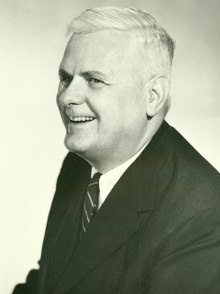
\includegraphics[width=3cm]{img/church}\\ \footnotesize Alonzo Church
\end{center}}{4cm}
\end{frame}

\begin{frame}{Idée}
L'idée de la programmation fonctionnelle est de recourir le plus possible aux fonctions et de faire en sorte que celle-ci ne produisent pas d'\textit{effets de bord} (traduction un peu trop littérale du terme Anglais \textit{side effect} qui signifie en réalité \textit{effet secondaire}).\\\pause

L'idée est qu'une fonction évaluée avec un jeu de paramètres doit \textit{toujours donner le même résultat.}
\end{frame}
\begin{frame}[fragile]{Effet de bord ?}
Voici un exemple de fonction induisant un effet de bord.
\inputminted{python}{scripts/func7.py}	
\end{frame}
\begin{frame}[fragile]{Quelle horreur !}
Il n'est pas acceptable que l'évaluation de \mintinline{python}{f(10)} donne deux valeurs différentes !\\\pause

Ainsi la programmation fonctionnelle interdit ce genre de fonctions.\\\pause 

L'effet de bord est dû au fait que le type \mintinline{python}{list} est \textit{mutable}, c'est-à-dire qu'on peut changer les éléments d'une liste après sa création.\\
\end{frame}

\begin{frame}[fragile]{Un problème ? Une solution...}
Pour contourner le problème, la programmation fonctionnelle interdit les types mutables.\\\pause

Dans un langage \textsc{Python} \textit{purement} fonctionnel, il n'y aurait pas de type \mintinline{python}{list}, simplement le type \mintinline{python}{tuple} (qui est non-mutable).\\
\end{frame}


\begin{frame}[fragile]{... Avec des conséquences notables !}
Suivant ce paradigme, l'exécution d'un programme est l'évaluation d'une ou plusieurs expressions, qui sont souvent des applications de fonctions à des valeurs passées en paramètre, tout en retenant bien que les fonctions elles-mêmes sont des valeurs.\\\pause 

La programmation fonctionnelle dite \textit{pure} bannit également l'idée de réaffectation : les variables créés et initialisées sont également non-mutables. C'est un peu comme si « les variables étaient des constantes».\\\pause

Hors de question d'écrire \mintinline{python}{i = i + 1} ou  bien même \mintinline{python}{for i in range(10)}. C'en est fini des boucles !\\
\end{frame}

\begin{frame}[fragile]{La catastrophe ?}
Dès lors on peut se demander s'il est vraiment possible de programmer suivant ce paradigme :\pause
\begin{enumerate}[--]
	\item 	pas d'effets de bord ;\pause 
	\item 	des variables non-mutables ;\pause
	\item 	pas de boucles.\pause 
\end{enumerate}
La réponse est oui, et on a démontré que l'on peut programmer autant de choses qu'en suivant les autres paradigmes que sont la POO ou la programmation impérative. Voici un exemple d'algorithme programmé en impératif puis en fonctionnel
\end{frame}

%%
\begin{frame}[fragile]{Version impérative}
\begin{minted}{python}
def somme(lst):
    s = 0
    for e in lst:
    	s = s + e
    return s

my_list = [1, 2, 3]
print(somme(my_list))
\end{minted}
\end{frame}

\begin{frame}[fragile]{Version fonctionnelle}
\begin{minted}[fontsize=\small]{python}
def somme(lst):
    return 0 if not lst else lst[0] + somme(lst[1:])

my_list = [1, 2, 3]
print(somme(my_list))
\end{minted}
\end{frame}

\begin{frame}{Analyse}
	On constate que le deuxième programme ne modifie aucune variable et ne contient pas de boucle, celle-ci a été remplacée par de la récursivité, c'est souvent le cas en programmation fonctionnelle.
\end{frame}

\begin{frame}{Avantages de la programmation fonctionnelle}
\begin{enumerate}[--]
	\item 	les programmes sont plus concis ;\pause
	\item 	on peut utiliser des \textit{fonctions d'ordre supérieur} c'est à dire des fonctions qui prennent d'autres fonctions en paramètre et/ou renvoient des fonctions en valeur de sortie ; \pause
	\item 	le fait qu'il n'y ait pas d'effets de bords rend les programmes \pause
	\begin{enumerate}[--]
		\item 	plus sûrs ; \pause 
		\item 	plus simple à débugger ; \pause
		\item 	plus simples à prouver. \pause
	\end{enumerate}
\end{enumerate}
\end{frame}
\end {document}